% How we do it: Why we do it, What particular method we use and what logic architecture we use
\section{The methodological approach}
\label{MethodApproach}
%---What methodology we used---

We analyze the possibility of automatically transform a BPEL written process in a Java executable routine, with minimum ad-hoc developer’s intervention. Our final objective is to show the feasibility of a semi-automated transformation from a small business process orchestrated with BPEL to the Java language.
This section describes the methodological approach we undertaken to realize our objective. The steps are summarized as following:

\begin{itemize}
 \item We identify the subset of BPEL instructions suitable for a proof of concept of the transformation.
 \item Select a BPEL meta-model that covers the chosen subset of instructions.
 \item Individuate a BPEL workflow pattern to work on
 \item Choose a model driven methodology that allows us to manipulate  the BPEL input model (M2M, M2T) and that is compatible with a ready to run code output.
\end{itemize} 

Once these steps have been accomplished, we focus on providing more details on how we carry out the transformation. The main points are:
\textbf{DA SCRIVERE NELLA SEZIONE DETAILED ARCHITECTURE ? }
\begin{itemize}
 \item Provide a correspondence from BPEL constructs to Java concepts
 \item Design the structure of the output application.
 \item Define the essential skeleton of Java classes necessary to create a runnable BPEL process
 \item In the templates, describe how to use and where the dynamic information taken from the BPEL input model has to be placed.
 \item Plan where and how, in the architecture, the developer intervention has to take place.
 \item \textbf{Issues encountered and proposed solutions  ? }
\end{itemize} 
 
 To mention later: \\
 StubPartnerLinks, code to be input by the user, static code, the problem with the WSDL file

\begin{figure}[h!]
  \begin{center}
    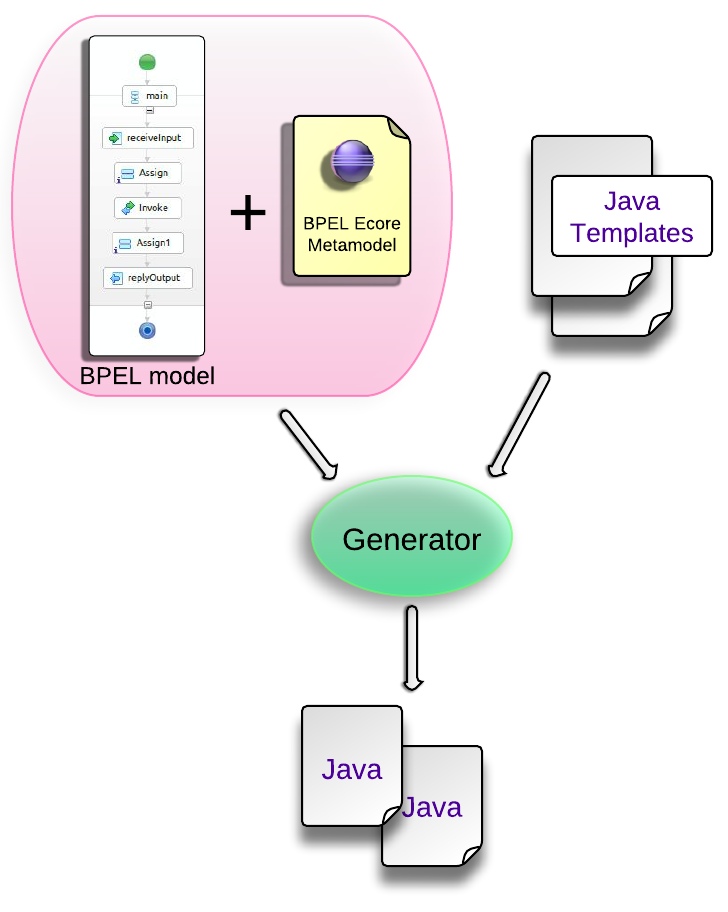
\includegraphics[scale=0.9]{pictures/TransformationApproach.png}
    \caption{Our methodological approach}
    \label{fig:TransformationApproach}
  \end{center}
\end{figure}